\section*{Introduction}
\addcontentsline{toc}{section}{Introduction}

This sprint report covers \textbf{Domain 5: AI Assistant \& Analytical Intelligence}. Building upon the complete shop-floor execution loop established in the previous sprints, this sprint delivers the AI layer of the MES system: a natural-language chat assistant embedded in the Flutter frontend, a \techname{Node.js} reverse proxy middleware that bridges the Flutter app to both \techname{Business Central} and a locally-hosted Python AI agent, and the Python agent itself. The agent provides deterministic tool orchestration, multi-provider LLM synthesis, fuzzy machine name resolution, multi-machine fan-out, production data enrichment, and contextual redirect actions. The result is a conversational interface that operators and supervisors can use to query real-time machine status, production orders, scrap rates, BOM consumption, delays, and operator performance without leaving the MES application.

% ---------------------------------------------------------------------------
% 1. SPRINT BACKLOG
% ---------------------------------------------------------------------------
\section{Sprint Backlog}

This sprint covers \textbf{Domain 5:} \textbf{\domainterm{AI Assistant \& Analytical Intelligence}}.

\begin{longtable}{@{} P{0.09\linewidth} P{0.38\linewidth} P{0.49\linewidth} @{}}
	\caption{US-5.1 --- AI Chat Interface}
	\label{tab:s5-US-5.1} \\
	\toprule
	\textbf{ID} & \textbf{User Story} & \textbf{Acceptance Criteria} \\
	\midrule
	\endfirsthead
	\toprule
	\textbf{ID} & \textbf{User Story} & \textbf{Acceptance Criteria} \\
	\midrule
	\endhead
	\multicolumn{3}{r}{\small Continued on next page} \\
	\endfoot
	\bottomrule
	\endlastfoot

	\textbf{US-5.1}
	& As an \userrole{Operator} or \userrole{Supervisor}, I need an embedded chat assistant in the MES app so that I can query production data using natural language without switching tools.
	& \noindent\textit{Flutter:}
	\begin{itemize}[noitemsep, topsep=0pt, partopsep=0pt, leftmargin=*]
		\item Create model \techname{ConversationTurn}, \techname{AiRedirectAction}, and \techname{AiChatResponse}.
		\item Create \techname{AiChatService} to POST to the \texttt{/api/ai/chat} endpoint.
		\item Create \techname{AiChatProvider} to manage conversation history, loading state, and the last response.
		\item Create page \techname{AiChatPage} supporting both modal dialog and embedded side-panel modes.
		\item Integrate the chat panel into \techname{MachineListPage} as a collapsible side panel on desktop and a modal dialog on mobile.
		\item Implement \techname{\_handleAction()} to process \techname{AiRedirectAction} objects (redirect to machine, operation, or machine list).
	\end{itemize} \\
	\midrule

	\textbf{US-5.2}
	& As a \userrole{Supervisor}, I need the AI to understand questions about multiple machines simultaneously so that I can get fleet-wide answers from a single query.
	& \noindent\textit{Python AI Agent:}
	\begin{itemize}[noitemsep, topsep=0pt, partopsep=0pt, leftmargin=*]
		\item Implement composite query detection in \modulename{composite.py}.
		\item Implement fan-out batch execution across machines using \texttt{asyncio.gather} in batches of 4.
		\item Implement \texttt{build\_composite\_context()} to produce a compact markdown context for the LLM.
		\item Cap fan-out at 12 machines to prevent timeout.
		\item Integrate the composite path into \techname{MESAgentOrchestrator}.
	\end{itemize} \\
	\midrule

	\textbf{US-5.3}
	& As an \userrole{Operator} or \userrole{Supervisor}, I need to refer to machines by colloquial names or partial identifiers so that I do not need to memorise exact machine codes.
	& \noindent\textit{Python AI Agent:}
	\begin{itemize}[noitemsep, topsep=0pt, partopsep=0pt, leftmargin=*]
		\item Implement \texttt{build\_machine\_index()} to build a lookup structure from the machine list.
		\item Implement a five-tier fuzzy resolution cascade in \texttt{resolve\_machine()} (exact canonical, normalised exact, digit suffix, ID prefix/suffix, token overlap, edit distance).
		\item Define \texttt{MIN\_CONFIDENCE = 0.45} and \texttt{HIGH\_CONFIDENCE = 0.85} thresholds.
		\item Implement \texttt{format\_candidates\_for\_llm()} to surface ambiguous matches to the user.
		\item Integrate resolver into orchestrator when \texttt{unresolved\_machine\_ref} is set.
	\end{itemize} \\
	\midrule

	\textbf{US-5.4}
	& As a \userrole{Supervisor}, I need the AI to alert me to overdue orders, excessive pauses, and high scrap rates so that I can take corrective action without manually reviewing dashboards.
	& \noindent\textit{Python AI Agent:}
	\begin{itemize}[noitemsep, topsep=0pt, partopsep=0pt, leftmargin=*]
		\item Implement \texttt{enrich\_deadlines()} in \modulename{data\_analysis.py} to compute \texttt{hours\_until\_deadline}, \texttt{is\_overdue}, and \texttt{risk\_level} per order.
		\item Implement \texttt{analyse\_scrap()} to compute \texttt{scrap\_rate}, \texttt{severity} (ok / warning / critical), \texttt{spike\_detected}, and \texttt{interpretation}.
		\item Implement \texttt{analyse\_velocity()} to compute \texttt{units\_per\_hour}, \texttt{required\_rate}, \texttt{projected\_end}, and \texttt{velocity\_status}.
		\item Wire enrichment results into the LLM context block before synthesis.
	\end{itemize} \\
	\midrule

	\textbf{US-5.5}
	& As an \userrole{Operator} or \userrole{Supervisor}, I need intent classification to work reliably without requiring a network call to an LLM so that the assistant remains responsive even when the LLM is slow.
	& \noindent\textit{Python AI Agent:}
	\begin{itemize}[noitemsep, topsep=0pt, partopsep=0pt, leftmargin=*]
		\item Implement \modulename{intent.py} with 12 intent classes and a priority-ordered regex rule cascade.
		\item Implement extraction helpers: \texttt{\_extract\_machine\_no()}, \texttt{\_extract\_machine\_ref()}, \texttt{\_extract\_order\_no()}, \texttt{\_extract\_op\_no()}, \texttt{\_extract\_hours()}.
		\item Define the \techname{ToolStep} and \techname{ToolChain} data types.
		\item Implement \modulename{llm\_intent.py} as the primary LLM-based classifier with automatic fallback to regex.
	\end{itemize} \\
	\midrule

	\textbf{US-5.6}
	& As a \userrole{Supervisor}, I need the AI to provide clickable navigation actions in its replies so that I can jump directly to a relevant machine or operation.
	& \noindent\textit{Python AI Agent:}
	\begin{itemize}[noitemsep, topsep=0pt, partopsep=0pt, leftmargin=*]
		\item Define the \techname{ActionType} enum with 5 redirect types in \modulename{models.py}.
		\item Implement \texttt{\_parse\_actions()} in the orchestrator to extract a \texttt{```actions```} JSON block from the LLM reply.
		\item Return up to 4 \techname{RedirectAction} objects in \techname{ChatResponse}.
	\end{itemize}
	\noindent\textit{Flutter:}
	\begin{itemize}[noitemsep, topsep=0pt, partopsep=0pt, leftmargin=*]
		\item Render \techname{\_ActionButtons} in \techname{AiChatPage} as a \texttt{Wrap} of tappable \texttt{ElevatedButton}s below each assistant reply.
		\item Implement \texttt{\_handleAction()} routing per action type.
	\end{itemize} \\

\end{longtable}

% ---------------------------------------------------------------------------
% 2. BUSINESS RULES
% ---------------------------------------------------------------------------
\section{Business Rules}

\Needspace{10\baselineskip}
\begin{longtable}{@{} P{0.30\linewidth} P{0.65\linewidth} @{}}
	\caption{Business Rules}
	\label{tab:s5-Business-Rules}\\
	\toprule
	\textbf{ID: Business Rule} & \textbf{Description} \\
	\midrule
	\endfirsthead
	\toprule
	\textbf{ID: Business Rule} & \textbf{Description} \\
	\midrule
	\endhead
	\multicolumn{2}{r}{\small Continued on next page} \\
	\endfoot
	\bottomrule
	\endlastfoot

	\multicolumn{2}{@{}l}{\textbf{AI Intent Classification Rules}} \\
	\midrule

	\businessrule{BR-AI-001}: Two-Tier Classification with Mandatory Fallback &
	The primary classifier (\modulename{llm\_intent.py}) sends a structured prompt to the LLM and validates the returned JSON plan against a schema. If the LLM response is malformed, missing required fields, references an unknown tool name, or contains duplicate \texttt{result\_key} values, the system falls back unconditionally to the deterministic regex classifier (\modulename{intent.py}). The fallback reason is recorded in the \domainterm{ThinkingBlock} but never surfaced to the end user. \\
	\midrule

	\businessrule{BR-AI-002}: LLM Does Not Control Tool Selection &
	The LLM's role is limited to producing a \emph{plan} (a list of tool names and arguments). Actual tool execution, access-control checks, slot resolution, and enrichment are performed entirely in Python. No tool is ever called solely on the LLM's instruction without passing through Python validation. This prevents prompt-injection attacks from influencing which data is fetched. \\
	\midrule

	\businessrule{BR-AI-003}: Exactly Two LLM Calls Per Request &
	Each \texttt{/chat} request triggers at most two LLM calls: one optional call in \texttt{LLMIntentIdentifier.classify()} for intent planning, and one mandatory call in \texttt{\_synthesise()} for response generation. The regex fallback path uses zero LLM calls for classification. Tool execution never triggers additional LLM calls. \\
	\midrule

	\multicolumn{2}{@{}l}{\textbf{Access Control Rules}} \\
	\midrule

	\businessrule{BR-AI-004}: Work-Center-Scoped Machine Access &
	The orchestrator builds an \texttt{allowed\_machines} dictionary by calling \texttt{ListMachinesTool} with the user's work centres extracted from the session token. Every subsequent call to a machine-scoped tool is checked against this dictionary before execution. If the requested machine is not in the allowed set, the tool call is skipped and an access-denial message is included in the context. The LLM never influences this check. \\
	\midrule

	\businessrule{BR-AI-005}: Token Forwarded to BC; Stripped from AI Calls &
	The session bearer token is included in the \texttt{user\_context} forwarded to the Python agent and is passed on to BC web service calls that require it (e.g., \texttt{fetchMyData}). The token is \emph{never} sent to the external LLM provider; it is only used for BC HTTP calls inside \modulename{mes\_tools.py}. \\
	\midrule

	\multicolumn{2}{@{}l}{\textbf{Machine Name Resolution Rules}} \\
	\midrule

	\businessrule{BR-AI-006}: Five-Tier Fuzzy Resolution with Confidence Thresholds &
	When a user refers to a machine by a colloquial name or partial ID, \modulename{resolver.py} applies a five-tier match cascade. A confidence score below \texttt{MIN\_CONFIDENCE = 0.45} causes the assistant to ask the user to clarify.
	\\ & 
	A score between 0.45 and \texttt{HIGH\_CONFIDENCE = 0.85} causes the assistant to proceed while noting the assumption. A score at or above 0.85 causes silent resolution. The five tiers are: (1) exact canonical ID, (2) normalised exact, (3) digit suffix match, (4) ID prefix/suffix overlap, and (5) token overlap and edit-distance scoring on the machine name. \\
	\midrule

	\multicolumn{2}{@{}l}{\textbf{Fan-Out Rules}} \\
	\midrule

	\businessrule{BR-AI-007}: Composite Queries Capped at 12 Machines &
	When a query is classified as composite (targeting multiple or all machines), \modulename{composite.py} filters the working set to the relevant machines (e.g., only Working machines for a running-status query), sorts them with Working machines first, and caps the fan-out at \texttt{MAX\_FANOUT\_MACHINES = 12}. Tool calls for the selected machines are dispatched in parallel batches of \texttt{BATCH\_SIZE = 4} using \texttt{asyncio.gather} to prevent BC from being overwhelmed. \\
	\midrule

	\multicolumn{2}{@{}l}{\textbf{Data Enrichment Rules}} \\
	\midrule

	\businessrule{BR-AI-008}: Pre-Computed Analytics Before LLM Synthesis &
	Numerical analysis (scrap rates, deadline risk levels, production velocity, utilisation percentages) is computed in Python by \modulename{data\_analysis.py} \emph{before} the LLM receives any data. The LLM is presented with pre-computed facts (e.g., \texttt{severity: "critical"}, \texttt{is\_overdue: true}) rather than raw numbers. This prevents numeric hallucination and ensures that alerts are deterministic. \\
	\midrule

	\multicolumn{2}{@{}l}{\textbf{Middleware Security Rules}} \\
	\midrule

	\businessrule{BR-MW-001}: SSPI Credential Isolation &
	The \techname{Node.js} middleware strips the Flutter \texttt{Authorization} header before forwarding any request to \techname{Business Central}. Authentication to BC is performed exclusively by the PowerShell child process using \texttt{UseDefaultCredentials = \$true}, which relies on the Windows session of the service account running the proxy. No BC credentials are stored in environment variables or configuration files accessible to the Node process. \\
	\midrule

	\businessrule{BR-MW-002}: SSPI Challenge Header Suppression &
	The \texttt{WWW-Authenticate} header returned by \techname{Business Central} during SSPI negotiation is stripped from all responses before they are forwarded to the Flutter client. This prevents the client from attempting to handle Kerberos/NTLM challenges that it has no capacity to process. \\
	\midrule

	\businessrule{BR-MW-003}: AI Route Priority &
	The Express middleware stack mounts \modulename{aiProxy.js} at \texttt{/api/ai} \emph{before} the BC catch-all handler \texttt{forwardRequest}. This ordering guarantees that no AI chat request ever reaches the PowerShell spawner. If \modulename{aiProxy.js} is removed or fails to load, the AI route falls through to the BC handler and returns an error rather than silently calling BC. \\
	\midrule

	\multicolumn{2}{@{}l}{\textbf{Conversation Rules}} \\
	\midrule

	\businessrule{BR-AI-009}: Conversation History Managed by Flutter &
	The \techname{AiChatProvider} maintains the full conversation history in memory as a \texttt{List<ConversationTurn>}. Each \texttt{/chat} call includes the history up to but not including the current turn. History is not persisted between application sessions. When the user clears the chat, history and the last response are both nulled. \\
	\midrule

	\businessrule{BR-AI-010}: LLM Context Capped Before Synthesis &
	The context block assembled from tool results and enrichment data is truncated to \texttt{LLM\_MAX\_CONTEXT\_CHARS} before being inserted into the synthesis prompt. This prevents token-limit errors regardless of how many machines or cycles were queried. The cap is configurable via an environment variable and defaults to a value defined in \modulename{config.py}. \\

\end{longtable}

% ---------------------------------------------------------------------------
% 3. DESIGN
% ---------------------------------------------------------------------------
\section{Design}

\subsection{Use Case Diagram}

This sprint adds a single new actor, the \domainterm{AI Assistant}, which mediates between the human user roles and the data layer. The primary use cases are: Chat with AI Assistant, Query Machine Status, Query Production Orders, Query Scrap Report, Query Operator Summary, Query Delay Report, Query BOM Consumption, Navigate to Machine (redirect action), and Navigate to Operation (redirect action).

Both the \userrole{Operator} and \userrole{Supervisor} roles can interact with the AI assistant for read-only queries scoped to their assigned work centres. The \userrole{Supervisor} additionally receives fleet-wide composite query results and supervisor-specific overview data. The resulting use case diagram is shown in Figure~\ref{fig:s5-use-case-diagram-s5}.

\begin{figure}[H]
  \centering
  
\includegraphics[width=\linewidth,keepaspectratio]{./media/MES_Sprint-5-Report/placeholder-image.png}
  \caption{UML Use Case Diagram --- Sprint 5}
  \label{fig:s5-use-case-diagram-s5}
\end{figure}

\subsection{Textual Use Case Description}

\Needspace{10\baselineskip}
\begin{longtable}{@{} P{0.21\linewidth} P{0.75\linewidth} @{}}
	\caption{Textual Use Case Description --- Chat with AI Assistant}
	\label{tab:s5-uc-chat} \\
	\toprule
	\endfirsthead
	\midrule
	\endhead
	\multicolumn{2}{r}{\small Continued on next page} \\
	\endfoot
	\bottomrule
	\endlastfoot

	\textbf{Use Case Name} & Chat with AI Assistant \\
	\midrule
	\textbf{Primary Actor} & \userrole{Operator} / \userrole{Supervisor} \\
	\midrule
	\textbf{Preconditions} &
	\begin{itemize}[noitemsep, topsep=0pt, partopsep=0pt, leftmargin=*]
	\item The user is authenticated and holds a valid session token.
	\item The AI chat panel is open (side panel on desktop, modal on mobile).
	\item The Node.js middleware and Python AI agent are running.
	\end{itemize} \\
	\midrule
	\textbf{Postconditions} &
	\begin{itemize}[noitemsep, topsep=0pt, partopsep=0pt, leftmargin=*]
	\item An assistant reply is appended to the conversation history.
	\item Up to 4 \domainterm{RedirectAction} buttons may be rendered below the reply.
	\item The conversation history is updated in \techname{AiChatProvider}.
	\end{itemize} \\
	\midrule
	\textbf{Main Scenario} &
	\begin{enumerate}[noitemsep, topsep=0pt, partopsep=0pt, leftmargin=*]
	\item The user types a message and taps the send button.
	\item \techname{AiChatProvider} appends a \domainterm{user} turn to the history and calls \texttt{AiChatService.sendMessage()}.
	\item The service POSTs to \apiendpoint{/api/ai/chat} with the message, user context (userId, role, work centres, token), and conversation history.
	\item The Node.js middleware routes the request to \apiendpoint{/api/ai} and forwards it to the Python AI agent.
	\item The AI agent classifies the intent, executes the tool chain against Business Central via the middleware, enriches the results, and synthesises a reply.
	\item The reply and optional redirect actions are returned as a \texttt{ChatResponse} JSON object.
	\item The Flutter UI appends the \domainterm{assistant} turn and renders any action buttons.
	\end{enumerate} \\
	\midrule
	\textbf{Alternative Flows} &
	\begin{itemize}[noitemsep, topsep=0pt, partopsep=0pt, leftmargin=*]
	\item \textit{LLM intent classification fails}: the regex classifier takes over; the user receives the same response with no visible difference.
	\item \textit{Machine name is ambiguous}: the assistant asks the user to clarify and lists the top candidate machines.
	\item \textit{AI agent timeout (60 s)}: the middleware returns a 504 error; the provider sets \texttt{errorMessage} and removes the failed user turn from history.
	\item \textit{Machine not in user's work centre}: the tool call is skipped; the assistant informs the user of the access restriction.
	\end{itemize} \\
\end{longtable}

\bigskip

\Needspace{10\baselineskip}
\begin{longtable}{@{} P{0.21\linewidth} P{0.75\linewidth} @{}}
	\caption{Textual Use Case Description --- Query Supervisor Overview}
	\label{tab:s5-uc-supervisor-overview} \\
	\toprule
	\endfirsthead
	\midrule
	\endhead
	\multicolumn{2}{r}{\small Continued on next page} \\
	\endfoot
	\bottomrule
	\endlastfoot

	\textbf{Use Case Name} & Query Supervisor Overview \\
	\midrule
	\textbf{Primary Actor} & \userrole{Supervisor} \\
	\midrule
	\textbf{Preconditions} &
	\begin{itemize}[noitemsep, topsep=0pt, partopsep=0pt, leftmargin=*]
	\item The user is authenticated with the \domainterm{Supervisor} role.
	\item The AI assistant is open.
	\end{itemize} \\
	\midrule
	\textbf{Postconditions} &
	\begin{itemize}[noitemsep, topsep=0pt, partopsep=0pt, leftmargin=*]
	\item The assistant returns a structured summary of stopped machines, idle operators, abnormal pauses, high-scrap operations, and delayed orders.
	\item Redirect actions allow the supervisor to navigate directly to flagged machines.
	\end{itemize} \\
	\midrule
	\textbf{Main Scenario} &
	\begin{enumerate}[noitemsep, topsep=0pt, partopsep=0pt, leftmargin=*]
	\item The supervisor types a broad query such as ``give me a shift overview''.
	\item The intent classifier maps the message to the \texttt{SUPERVISOR\_OVERVIEW} intent.
	\item The orchestrator calls \texttt{GetSupervisorOverviewTool} which in turn calls \apiendpoint{fetchSupervisorOverview} on the BC web service.
	\item The returned JSON (stopped machines, idle operators, abnormal pauses, high-scrap operations, delayed orders) is enriched with delay risk levels by \modulename{data\_analysis.py}.
	\item The LLM synthesises a concise shift report and emits up to 4 redirect actions pointing to the most critical machines.
	\item The supervisor taps a redirect action to navigate directly to the flagged machine page.
	\end{enumerate} \\
\end{longtable}

\subsection{Sequence Diagrams}

The following sequence diagrams illustrate the communication flow between the \techname{Flutter} frontend, the \techname{Node.js} middleware, the \techname{Python AI Agent}, and \techname{Business Central} for the primary AI interaction flows.

Figure~\ref{fig:s5-seq-ai-chat} depicts the main chat flow: the Flutter client sends a message with user context to the middleware, which routes it to the Python agent. The agent classifies the intent, executes the BC tool chain via the middleware's PowerShell proxy, enriches the results, and synthesises a reply using the configured LLM.

\begin{figure}[H]
  \centering
  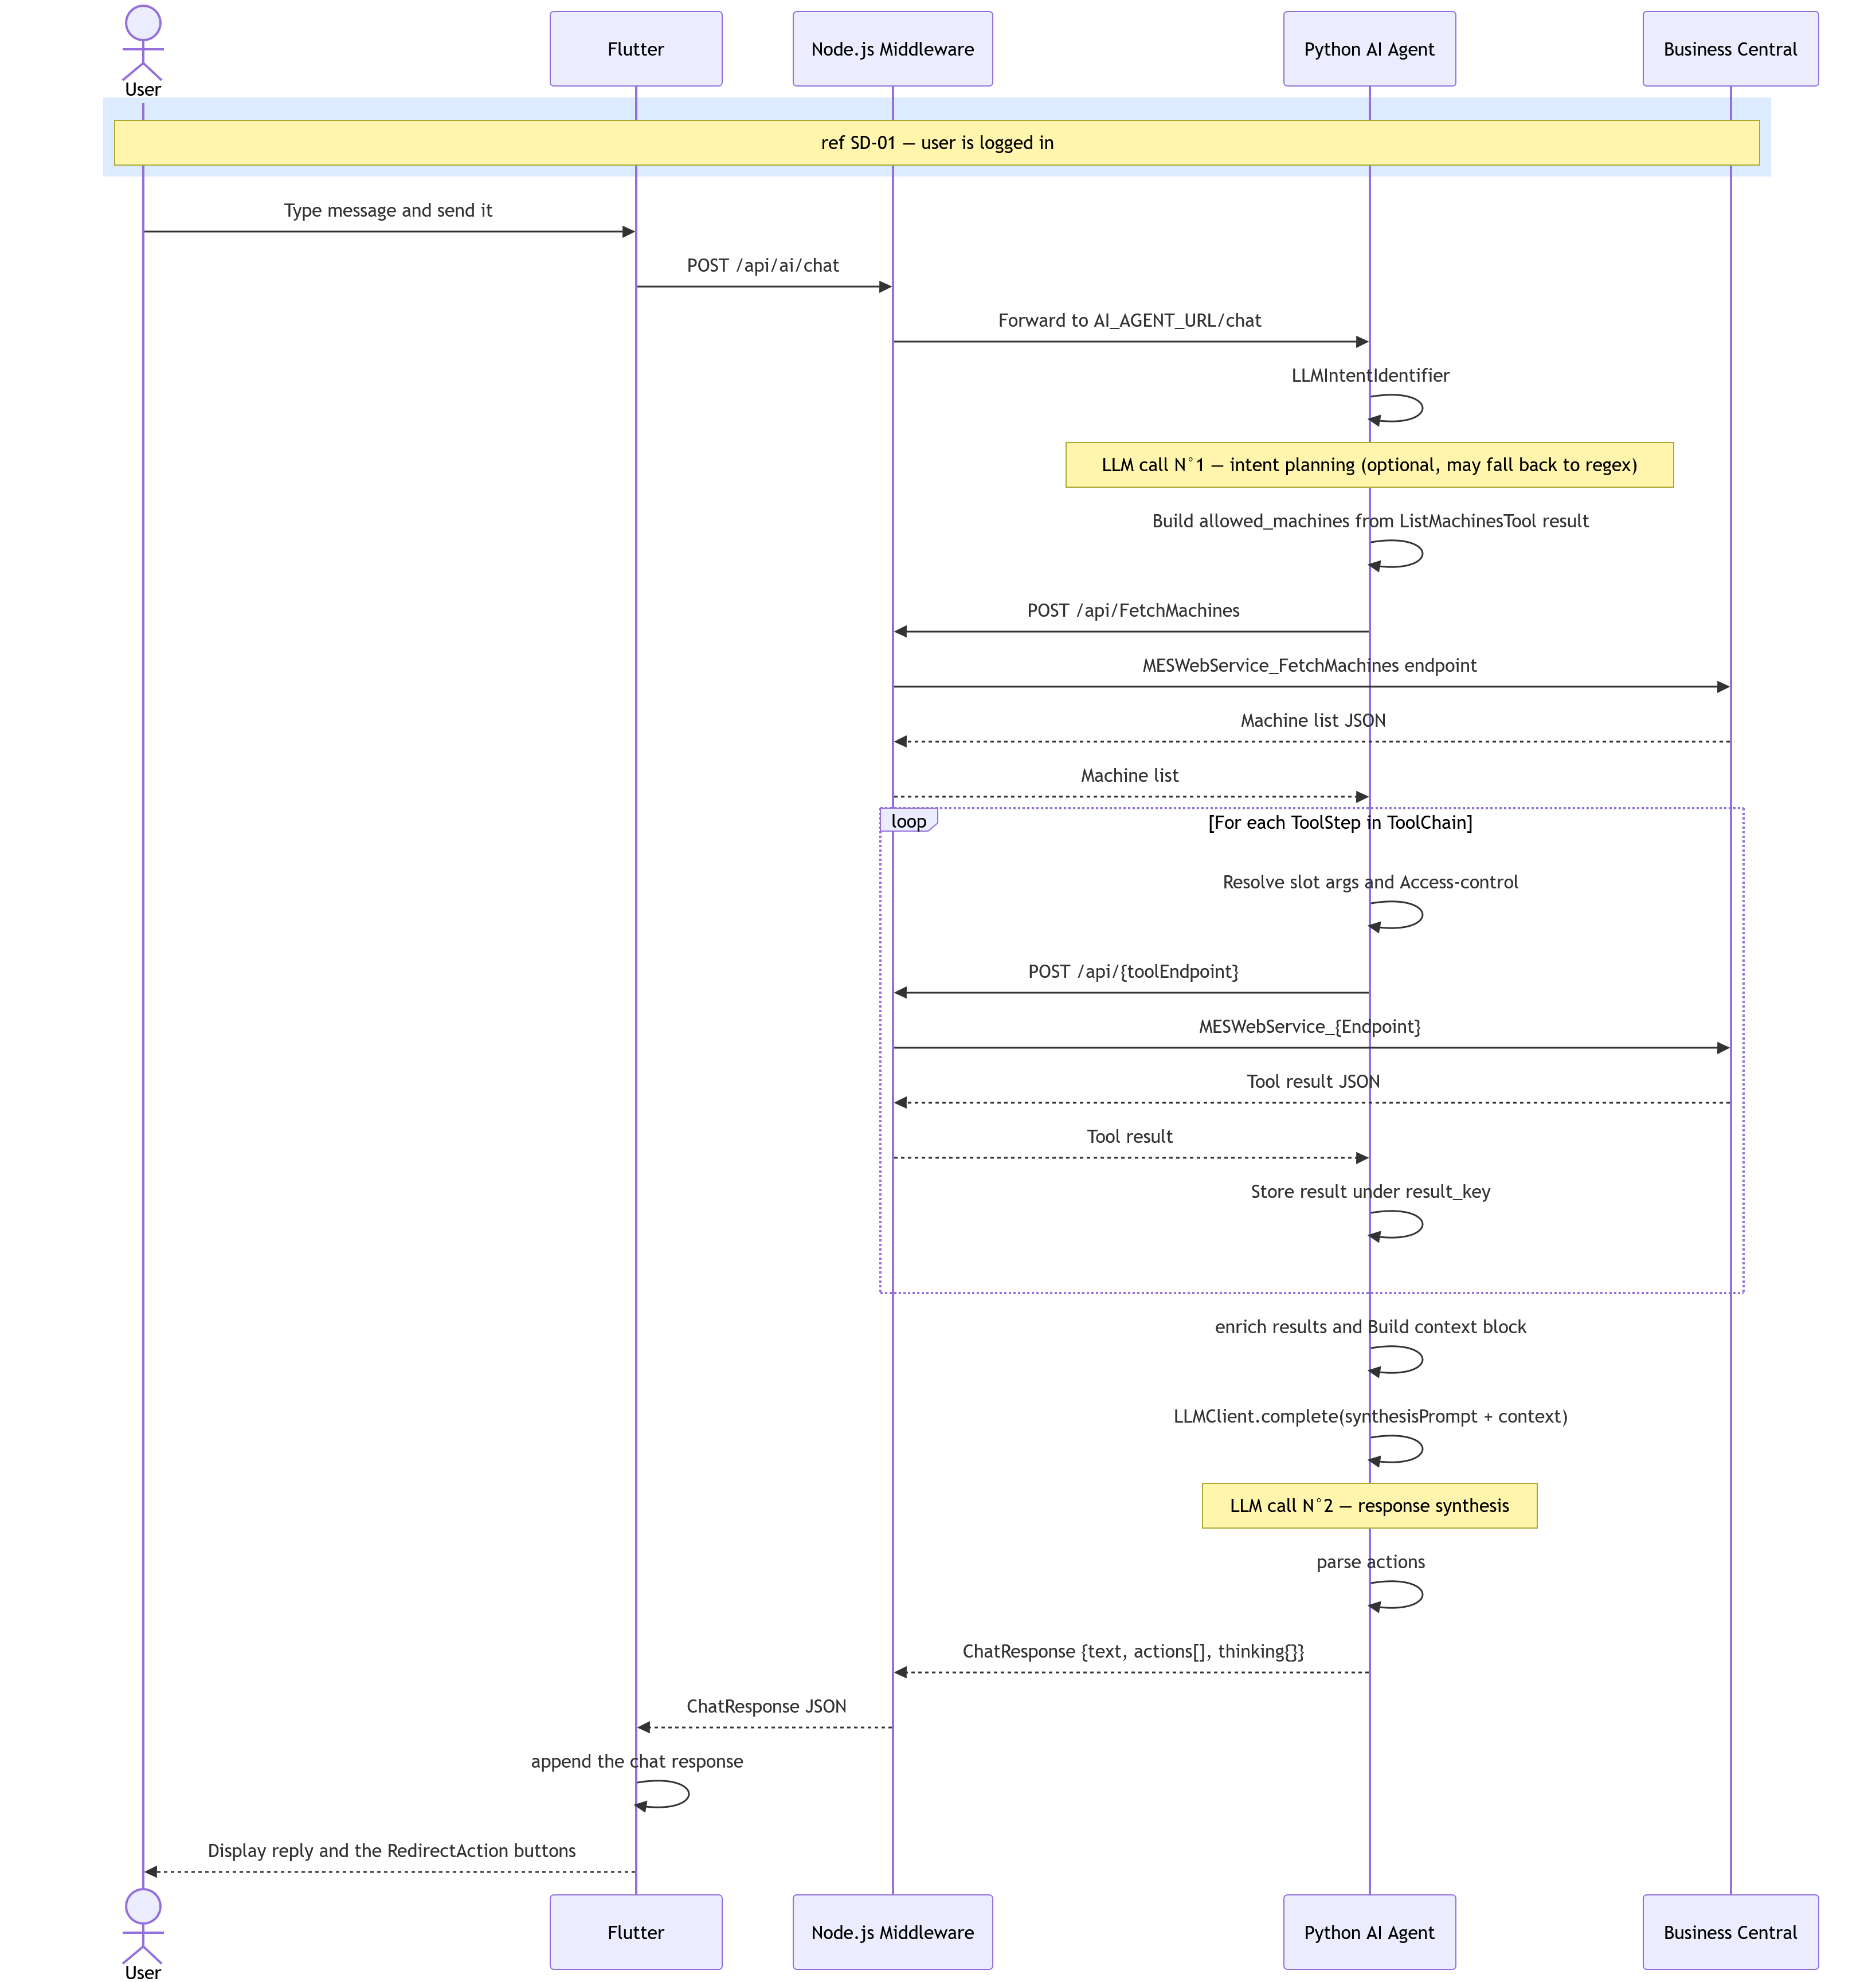
\includegraphics[width=\linewidth,height=0.82\textheight,keepaspectratio]{./media/MES_Sprint-5-Report/diagrams/sequence/AIChat-MainFlow.png}
  \caption{SD-30: AI Chat --- Main Flow.}
  \label{fig:s5-seq-ai-chat}
\end{figure}
%=====SD-30==========================================================
% sequenceDiagram
%     actor User
%     participant Flutter
%     participant Node as Node.js Middleware
%     participant Agent as Python AI Agent
%     participant BC as Business Central

%     rect rgb(220,235,255)
%         Note over User,BC: ref SD-01 — user is logged in
%     end

%     User->>Flutter: Type message and send it
%     Flutter->>Node: POST /api/ai/chat

%     Node->>Agent: Forward to AI_AGENT_URL/chat

%     Agent->>Agent: LLMIntentIdentifier
%     Note over Agent: LLM call N°1 — intent planning (optional, may fall back to regex)

%     Agent->>Agent: Build allowed_machines from ListMachinesTool result
%     Agent->>Node: POST /api/FetchMachines
%     Node->>BC: MESWebService_FetchMachines endpoint 
%     BC-->>Node: Machine list JSON
%     Node-->>Agent: Machine list

%     loop For each ToolStep in ToolChain
%         Agent->>Agent: Resolve slot args and Access-control
%         Agent->>Node: POST /api/{toolEndpoint}
%         Node->>BC: MESWebService_{Endpoint}
%         BC-->>Node: Tool result JSON
%         Node-->>Agent: Tool result
%         Agent->>Agent: Store result under result_key
%     end

%     Agent->>Agent: enrich results and Build context block

%     Agent->>Agent: LLMClient.complete(synthesisPrompt + context)
%     Note over Agent: LLM call N°2 — response synthesis

%     Agent->>Agent: parse actions
%     Agent-->>Node: ChatResponse {text, actions[], thinking{}}
%     Node-->>Flutter: ChatResponse JSON

%     Flutter->>Flutter: append the chat response
%     Flutter-->>User: Display reply and the RedirectAction buttons
%====================================================================

Figure~\ref{fig:s5-seq-intent-classification} illustrates the two-tier intent classification flow, showing the LLM-based primary classifier, the JSON plan validation step, and the fallback path to the regex classifier. The \domainterm{ThinkingBlock} capturing the classification trace is also shown.

\begin{figure}[H]
  \centering
  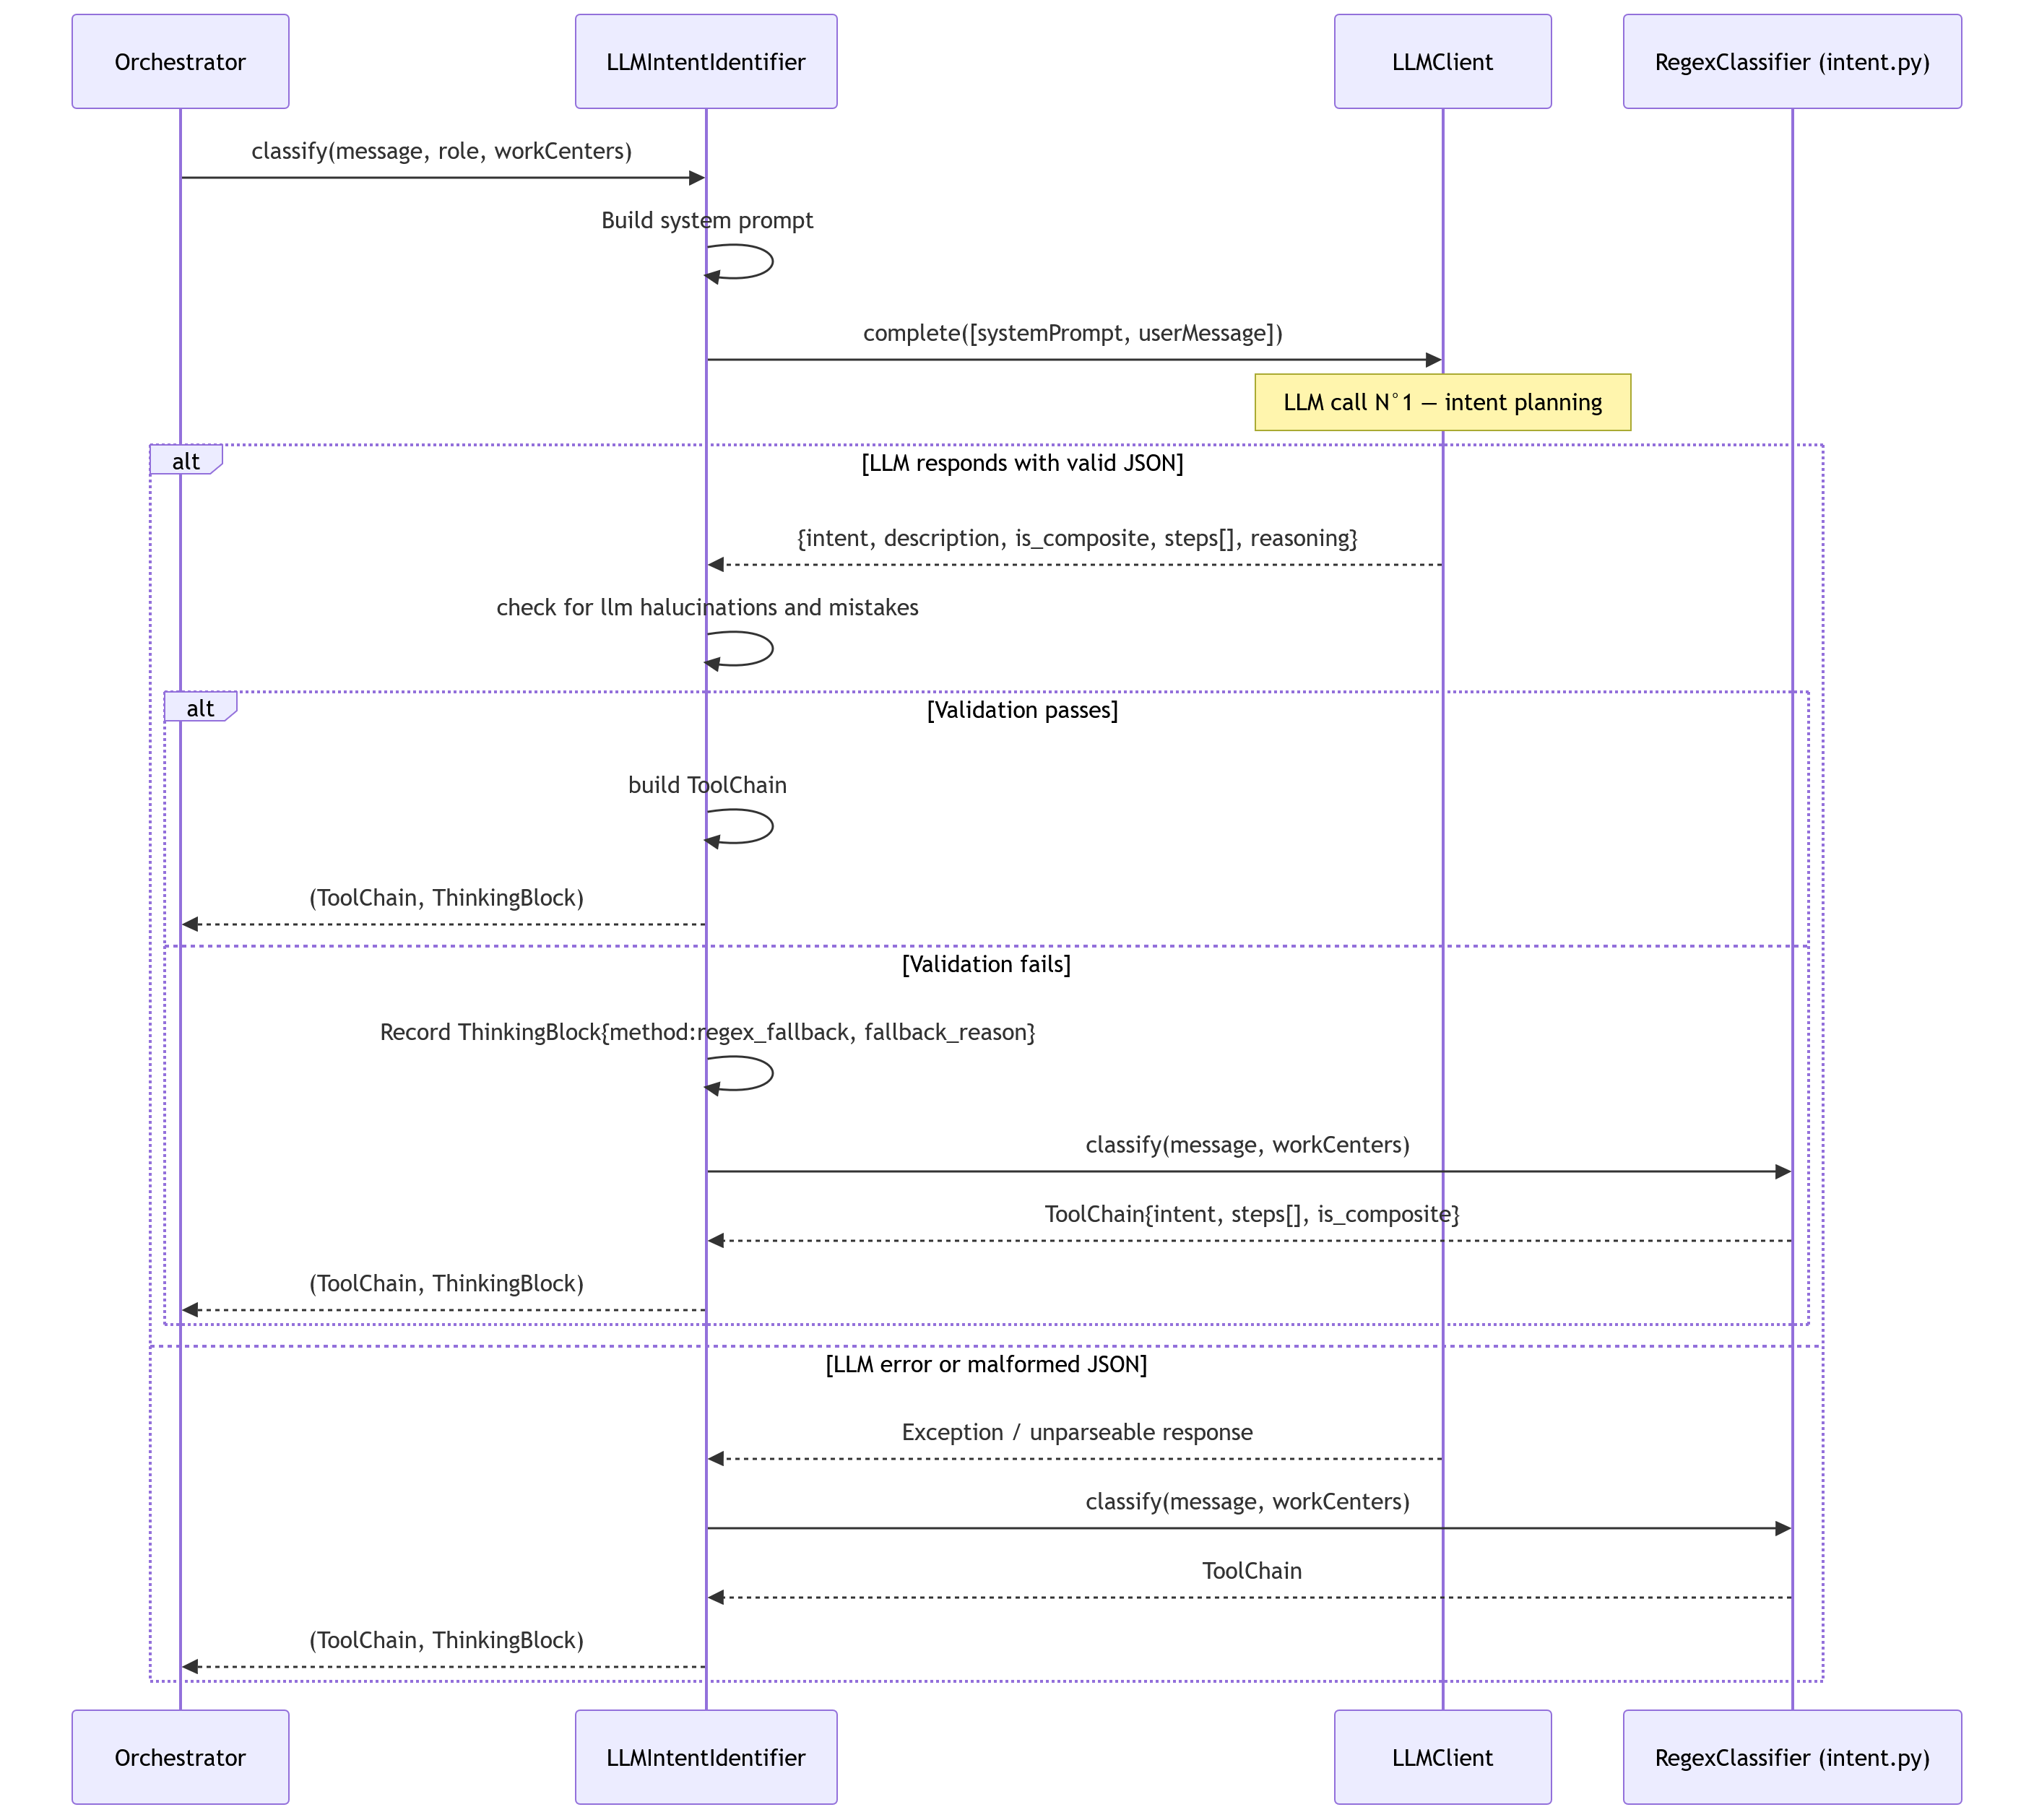
\includegraphics[width=\linewidth,height=0.82\textheight,keepaspectratio]{./media/MES_Sprint-5-Report/diagrams/sequence/Intent-Classification.png}
  \caption{SD-31: Intent Classification --- LLM with Regex Fallback.}
  \label{fig:s5-seq-intent-classification}
\end{figure}

% sequenceDiagram
%     participant Orch as Orchestrator
%     participant LLMIntent as LLMIntentIdentifier
%     participant LLMClient as LLMClient
%     participant Regex as RegexClassifier (intent.py)

%     Orch->>LLMIntent: classify(message, role, workCenters)

%     LLMIntent->>LLMIntent: Build system prompt
%     LLMIntent->>LLMClient: complete([systemPrompt, userMessage])
%     Note over LLMClient: LLM call N°1 — intent planning

%     alt LLM responds with valid JSON
%         LLMClient-->>LLMIntent: {intent, description, is_composite, steps[], reasoning}
%         LLMIntent->>LLMIntent: check for llm halucinations and mistakes
%         alt Validation passes
%             LLMIntent->>LLMIntent: build ToolChain
%             LLMIntent-->>Orch: (ToolChain, ThinkingBlock)
%         else Validation fails
%             LLMIntent->>LLMIntent: Record ThinkingBlock{method:regex_fallback, fallback_reason}
%             LLMIntent->>Regex: classify(message, workCenters)
%             Regex-->>LLMIntent: ToolChain{intent, steps[], is_composite}
%             LLMIntent-->>Orch: (ToolChain, ThinkingBlock)
%         end
%     else LLM error or malformed JSON
%         LLMClient-->>LLMIntent: Exception / unparseable response
%         LLMIntent->>Regex: classify(message, workCenters)
%         Regex-->>LLMIntent: ToolChain
%         LLMIntent-->>Orch: (ToolChain, ThinkingBlock)
%     end

\subsection{Class Diagram}

The UML Class Diagram (Figure~\ref{fig:s5-class-diagram-s5}) shows the Python AI agent's domain model. \modulename{MES Agent Orchestrator} is the central coordinator, holding references to an \modulename{LLM Intent Identifier}, an \modulename{LLM Client} (the abstract interface implemented by six concrete provider classes), and the \modulename{TOOL MAP} registry. \modulename{Tool Chain} is a value object produced by the classifiers and consumed by the orchestrator; it contains an ordered list of \modulename{Tool Step} records. All tool classes implement a common \texttt{execute()} interface. \modulename{Chat Request} and \modulename{Chat Response} are the inbound and outbound Pydantic contracts of the \texttt{/chat} endpoint.

\begin{figure}[H]
  \centering
  
\includegraphics[width=\linewidth,keepaspectratio]{./media/MES_Sprint-5-Report/placeholder-image.png}
  \caption{UML Class Diagram --- AI Assistant \& Analytical Intelligence.}
  \label{fig:s5-class-diagram-s5}
\end{figure}

% ---------------------------------------------------------------------------
% 4. IMPLEMENTATION
% ---------------------------------------------------------------------------
\section{Implementation}

\subsection{Python AI Agent}

\subsubsection{Data Models}

\begin{longtable}{@{} P{0.25\linewidth} P{0.25\linewidth} P{0.45\linewidth} @{}}
	\caption{Pydantic Models --- \modulename{agent/models.py}}
	\label{tab:s5-pydantic-models} \\
	\toprule
	\textbf{Class} & \textbf{Key Fields} & \textbf{Description} \\
	\midrule
	\endfirsthead
	\toprule
	\textbf{Class} & \textbf{Key Fields} & \textbf{Description} \\
	\midrule
	\endhead
	\multicolumn{3}{r}{\small Continued on next page} \\
	\endfoot
	\bottomrule
	\endlastfoot

	\techname{ConversationTurn} & \texttt{role}, \texttt{content} & One message in the conversation history. Role is either \texttt{"user"} or \texttt{"assistant"}. \\
	\midrule
	\techname{UserContext} & \texttt{user\_id}, \texttt{role}, \texttt{work\_centers}, \texttt{token} & Session identity extracted from the Flutter session storage and forwarded with every chat request. \\
	\midrule
	\techname{ChatRequest} & \texttt{message}, \texttt{user\_context}, \texttt{conversation\_history} & Inbound contract for the \texttt{POST /chat} endpoint. \texttt{conversation\_history} defaults to an empty list. \\
	\midrule
	\techname{ActionType} & enum: 5 values & Defines the five redirect types the LLM may emit: \texttt{redirect\_machine}, \texttt{redirect\_operation}, \texttt{redirect\_machine\_list}, and two reserved types. \\
	\midrule
	\techname{RedirectAction} & \texttt{action\_type}, \texttt{label}, \texttt{payload} & A clickable navigation action sent back to Flutter and rendered as an \texttt{ElevatedButton}. \\
	\midrule
	\techname{ChatResponse} & \texttt{text}, \texttt{actions}, \texttt{data\_fetched}, \texttt{thinking} & Outbound contract. \texttt{text} is the human-readable reply; \texttt{actions} holds up to 4 redirect actions; \texttt{thinking} carries the classification trace for debugging. \\
	\midrule
	\techname{ToolResult} & \texttt{tool\_name}, \texttt{success}, \texttt{data}, \texttt{error} & Internal result wrapper returned by every tool's \texttt{execute()} method. \\
\end{longtable}

\subsubsection{Intent Classification}

The intent classification layer comprises two components working in tandem. \modulename{llm\_intent.py} is the primary classifier: it sends a terse system prompt listing all 17 available tools to the configured LLM and expects a JSON response containing the \texttt{intent} label, a \texttt{steps} array, and an optional \texttt{reasoning} field. This plan is validated by \texttt{\_validate\_plan()}, which checks that the intent label is known, all tool names exist in \texttt{TOOL\_MAP}, and no \texttt{result\_key} is duplicated across steps.

If validation fails for any reason — malformed JSON, unknown tool, missing required field — control passes to \modulename{intent.py}, the deterministic regex classifier. Table~\ref{tab:s5-intent-classes} lists the 12 intent classes and their primary trigger patterns.

\begin{longtable}{@{} P{0.28\linewidth} P{0.67\linewidth} @{}}
	\caption{Intent Classes --- \modulename{agent/intent.py}}
	\label{tab:s5-intent-classes} \\
	\toprule
	\textbf{Intent} & \textbf{Primary Trigger Patterns} \\
	\midrule
	\endfirsthead
	\toprule
	\textbf{Intent} & \textbf{Primary Trigger Patterns} \\
	\midrule
	\endhead
	\multicolumn{2}{r}{\small Continued on next page} \\
	\endfoot
	\bottomrule
	\endlastfoot

	\texttt{BOM} & \textit{bom}, \textit{component}, \textit{material}, \textit{consumption}, \textit{scan} \\
	\midrule
	\texttt{PRODUCTION\_CYCLES} & \textit{cycle}, \textit{declaration}, \textit{declared}, \textit{production history} \\
	\midrule
	\texttt{OPERATION\_LIVE} & \textit{live}, \textit{current operation}, \textit{running}, \textit{in progress} \\
	\midrule
	\texttt{OPERATION\_HISTORY} & \textit{history}, \textit{past operation}, \textit{finished}, \textit{cancelled} \\
	\midrule
	\texttt{ORDERS} & \textit{order}, \textit{production order}, \textit{PO-}, \textit{scheduled} \\
	\midrule
	\texttt{MACHINE\_LIVE} & \textit{machine status}, \textit{what is MC-}, \textit{ongoing} \\
	\midrule
	\texttt{DASHBOARD} & \textit{dashboard}, \textit{summary}, \textit{overview}, \textit{KPI} \\
	\midrule
	\texttt{MACHINE\_STATUS} & \textit{idle}, \textit{working}, \textit{which machines are} \\
	\midrule
	\texttt{SCRAP\_ANALYSIS} & \textit{scrap}, \textit{reject}, \textit{waste}, \textit{defect} \\
	\midrule
	\texttt{ACTIVITY} & \textit{activity}, \textit{event log}, \textit{what happened}, \textit{recent actions} \\
	\midrule
	\texttt{DEPARTMENT} & \textit{work center}, \textit{department}, \textit{sector}, \textit{operator summary} \\
	\midrule
	\texttt{GENERAL} & Catch-all when no higher-priority rule matches. \\
\end{longtable}

\subsubsection{Tool Catalogue}

Table~\ref{tab:s5-tool-catalogue} lists all 17 tool classes registered in \texttt{TOOL\_MAP}, together with the \techname{Business Central} endpoint each tool calls and its primary arguments.

\begin{longtable}{@{} P{0.32\linewidth} P{0.30\linewidth} P{0.33\linewidth} @{}}
	\caption{MES Tool Catalogue --- \modulename{tools/mes\_tools.py}}
	\label{tab:s5-tool-catalogue} \\
	\toprule
	\textbf{Tool Class} & \textbf{BC Endpoint} & \textbf{Key Arguments} \\
	\midrule
	\endfirsthead
	\toprule
	\textbf{Tool Class} & \textbf{BC Endpoint} & \textbf{Key Arguments} \\
	\midrule
	\endhead
	\multicolumn{3}{r}{\small Continued on next page} \\
	\endfoot
	\bottomrule
	\endlastfoot

	\techname{ListMachinesTool} & \texttt{FetchMachines} & \texttt{work\_center\_no} \\
	\midrule
	\techname{GetMachineOrdersTool} & \texttt{getMachineOrders} & \texttt{machine\_no} \\
	\midrule
	\techname{GetOngoingOperationsTool} & \texttt{fetchOngoing-\linebreak OperationsState} & \texttt{machine\_no} \\
	\midrule
	\techname{GetOperationLiveDataTool} & \texttt{fetchOperationLiveData} & \texttt{machine\_no}, \texttt{prod\_order\_no}, \texttt{operation\_no} \\
	\midrule
	\techname{GetProductionCyclesTool} & \texttt{fetchProductionCycles} & \texttt{machine\_no}, \texttt{prod\_order\_no}, \texttt{operation\_no} \\
	\midrule
	\techname{GetOperationsHistoryTool} & \texttt{fetchOperationsHistory} & \texttt{machine\_no} \\
	\midrule
	\techname{GetActivityLogTool} & \texttt{fetchActivityLog} & \texttt{hours\_back} \\
	\midrule
	\techname{GetMachineDashboardTool} & \texttt{fetchMachineDashboard} & \texttt{hours\_back}, \texttt{work\_center\_nos} \\
	\midrule
	\techname{GetProductionOrdersTool} & \texttt{fetchProductionOrders} & \texttt{status\_filter}, \texttt{work\_center\_no}, \texttt{machine\_no} \\
	\midrule
	\techname{GetWorkCenterSummaryTool} & \texttt{fetchWorkCenterSummary} & \texttt{work\_center\_nos}, \texttt{hours\_back} \\
	\midrule
	\techname{GetOperatorSummaryTool} & \texttt{fetchOperatorSummary} & \texttt{work\_center\_nos}, \texttt{hours\_back} \\
	\midrule
	\techname{GetMyDataTool} & \texttt{fetchMyData} & \texttt{hours\_back} (token-scoped) \\
	\midrule
	\techname{GetScrapSummaryTool} & \texttt{fetchScrapSummary} & \texttt{hours\_back}, multi-filter \\
	\midrule
	\techname{GetDelayReportTool} & \texttt{fetchDelayReport} & \texttt{work\_center\_nos}, \texttt{pause\_threshold\_minutes} \\
	\midrule
	\techname{GetConsumptionSummaryTool} & \texttt{fetchConsumptionSummary} & \texttt{prod\_order\_no}, \texttt{operation\_no}, \texttt{machine\_no}, \texttt{hours\_back} \\
	\midrule
	\techname{GetSupervisorOverviewTool} & \texttt{fetchSupervisorOverview} & \texttt{work\_center\_nos}, \texttt{hours\_back}, \texttt{pause\_threshold\_minutes} \\
	\midrule
	\techname{GetBomTool} & \texttt{fetchBom} & \texttt{prod\_order\_no}, \texttt{operation\_no} \\
\end{longtable}

\subsubsection{Orchestration Pipeline}

\techname{MESAgentOrchestrator.run()} processes each \texttt{ChatRequest} through an eight-step pipeline. Step 1 calls \texttt{LLMIntentIdentifier.classify()} (with regex fallback) to produce a \texttt{ToolChain}. Step 2 routes to the composite path (if \texttt{is\_composite = true}) or the normal sequential path. Step 3 resolves any \texttt{unresolved\_machine\_ref} using \modulename{resolver.py}. Step 4 iterates the tool steps: slot arguments prefixed with \texttt{\$} are resolved against prior step results, access-control is verified against \texttt{allowed\_machines}, and the tool is executed. Step 5 applies \modulename{data\_analysis.py} enrichment per result key. Step 6 assembles the LLM context block and truncates it to \texttt{LLM\_MAX\_CONTEXT\_CHARS}. Step 7 calls the LLM once for synthesis. Step 8 extracts any \texttt{```actions```} block from the reply and separates it from the displayed text.

\subsubsection{Multi-Provider LLM Client}

The \texttt{build\_llm\_client()} factory reads the \texttt{LLM\_PROVIDER} environment variable and instantiates the corresponding client class. All clients expose the same \texttt{async complete(messages: list) → str} interface so the rest of the agent is provider-agnostic. Table~\ref{tab:s5-llm-providers} summarises the supported providers.

\begin{longtable}{@{} P{0.30\linewidth} P{0.30\linewidth} P{0.35\linewidth} @{}}
	\caption{Supported LLM Providers --- \modulename{agent/llm\_client.py}}
	\label{tab:s5-llm-providers} \\
	\toprule
	\textbf{Client Class} & \textbf{Provider} & \textbf{Notes} \\
	\midrule
	\endfirsthead
	\toprule
	\textbf{Client Class} & \textbf{Provider} & \textbf{Notes} \\
	\midrule
	\endhead
	\multicolumn{3}{r}{\small Continued on next page} \\
	\endfoot
	\bottomrule
	\endlastfoot

	\techname{OllamaClient} & Local Ollama & No external credential required; model served locally. \\
	\midrule
	\techname{OpenAIClient} & OpenAI & Requires \texttt{OPENAI\_API\_KEY}. \\
	\midrule
	\techname{HuggingFaceClient} & HF Serverless Inference & Requires \texttt{HF\_API\_TOKEN}. \\
	\midrule
	\techname{OpenAICompatibleClient} & Groq, Together, Mistral, vLLM, LM Studio & Uses the OpenAI Chat Completions schema with a configurable base URL. \\
	\midrule
	\techname{AnthropicClient} & Anthropic & Extracts the system prompt from the messages list before calling the Messages API. \\
\end{longtable}

\subsection{Node.js Middleware}

\subsubsection{Endpoint Routing}

We configured the middleware to map all calls coming from the frontend using the structure \techname{/api/ai} to the ai proxy handler which forwards them to the \techname{/chat} endpoint of the Python agent. The agents tool calls are treated through the same path as the normal business central function calls by the flutter frontend.

\subsection{Flutter Frontend}

\subsubsection{AI Data Layer}

The Flutter data layer for the AI feature comprises three classes. \techname{AiChatService} constructs the full request payload — including user context assembled from \techname{SessionStorage} at call time — and POSTs it to \apiendpoint{/api/ai/chat}. It deserialises the response into an \techname{AiChatResponse} object. \techname{ConversationTurn} is a minimal data class with \texttt{role} and \texttt{content} fields and a \texttt{toJson()} serialiser. \techname{AiChatResponse} holds the reply text, the list of \techname{AiRedirectAction} objects, and an optional error string.

\subsubsection{AI Domain Layer}

\techname{AiChatProvider} extends \texttt{ChangeNotifier} and owns the conversation history as a \texttt{List\linebreak<ConversationTurn>}. Its \texttt{sendMessage()} method appends the user turn before calling the service, and on success appends the assistant turn and stores \texttt{lastResponse}. On failure it removes the failed user turn and sets \texttt{errorMessage}. \texttt{clearHistory()} resets both the history and the last response, enabling the user to start a fresh conversation.

\subsubsection{User Interface}

Figure~\ref{fig:s5-ui-ai-chat-mobile} illustrate the \uilabel{AI Chat} interface in its two display modes. On desktop (width $\geq$ 600 px), the chat panel opens as a 400 px fixed-width side panel anchored to the right of the \uilabel{Machine List Page}, and the floating action button (FAB) is hidden while the panel is open. On mobile, the chat opens as a full \texttt{Dialog} widget (max 800$\times$800 px). In both modes the interface comprises the same four sub-widgets: \techname{\_EmptyState} (shown before the first message), \techname{\_MessageBubble} (dark background for user turns, light grey for assistant turns, capped at 78\% of available width), \techname{\_ActionButtons} (a \texttt{Wrap} of \texttt{ElevatedButton}s for each \techname{RedirectAction}), and \techname{\_InputBar} (a \texttt{TextField} with a send icon button that switches to a \texttt{CircularProgressIndicator} while a request is in flight).
% empty state
\begin{figure}[H]
  \centering
  
\includegraphics[width=0.5\linewidth,keepaspectratio]{./media/MES_Sprint-5-Report/placeholder-image.png}
  \caption{\uilabel{AI Chat} dialog --- mobile view.}
  \label{fig:s5-ui-ai-chat-mobile-empty}
\end{figure}


% message state don't forget to add a redirect action
\begin{figure}[H]
  \centering
  
\includegraphics[width=0.5\linewidth,keepaspectratio]{./media/MES_Sprint-5-Report/placeholder-image.png}
  \caption{\uilabel{AI Chat} dialog --- mobile view.}
  \label{fig:s5-ui-ai-chat-mobile}
\end{figure}

% ---------------------------------------------------------------------------
% CONCLUSION
% ---------------------------------------------------------------------------
\phantomsection
\section*{Conclusion}
\addcontentsline{toc}{section}{Conclusion}

This sprint delivered the complete AI intelligence layer of the MES system. Operators and supervisors can now query production data, machine status, scrap rates, BOM consumption, operator performance, and shift overviews using natural language through the embedded chat assistant. The two-tier intent classification architecture — LLM-based planning with deterministic regex fallback — ensures reliable and responsive behaviour regardless of LLM availability. Work-centre-scoped access control, implemented entirely in Python and independent of LLM output, guarantees that users can only query data within their authorised scope. The multi-provider LLM client makes the system adaptable to different deployment environments, from a locally-hosted Ollama model to cloud providers such as Anthropic or OpenAI. The \techname{Node.js} middleware resolves the SSPI authentication challenge inherent to \techname{Business Central}'s OData layer while keeping the Flutter client and Python agent free of Windows-specific dependencies. Together, these components form a production-ready conversational intelligence layer that integrates seamlessly with the shop-floor execution features delivered in the preceding sprints.
